\chapter{Motion measurements II: \\Feature plots}\label{cha:matlabFeaturesPlot}
In the result of motion measurements II (~\sectionref{res:testII}, plots were scattered to analyze which features that are most suitable for device fingerprinting. This appendix includes these plots that are used in~\sectionref{res:testII} and discussed in~\sectionref{sec:concl:acc}.

\section{Scatter-plot of mean values}
\begin{figure}[H]
	\centering
	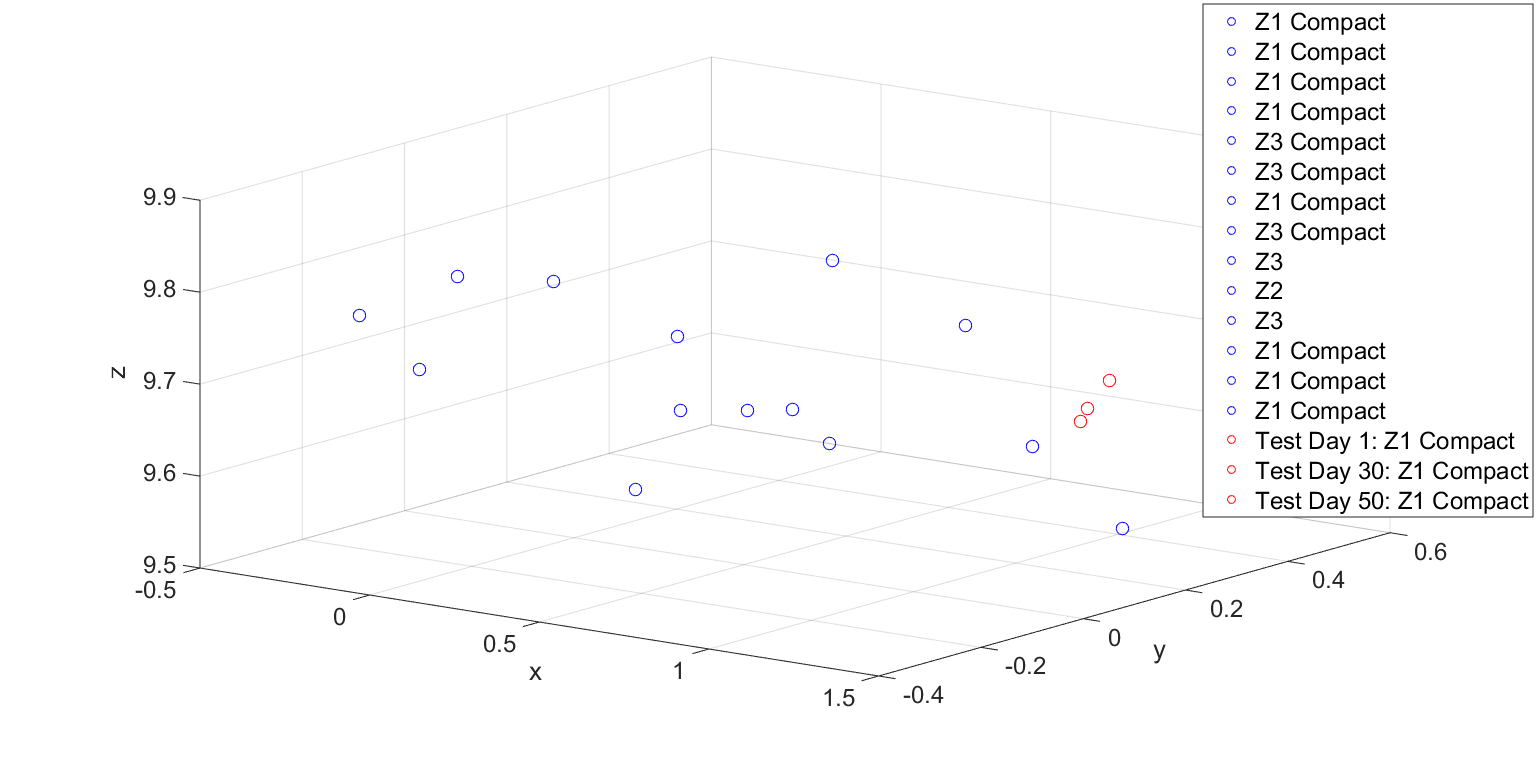
\includegraphics[scale=.3]{img/features/mean}
	\caption{Scatter-plot of mean values of 12  \textit{Sony Xperia Z}-devices including one device with readings over a period of 50 days}
	\label{fig:feature:mean}
\end{figure}

\section{Scatter-plot of standard deviation values}
\begin{figure}[H]
	\centering
	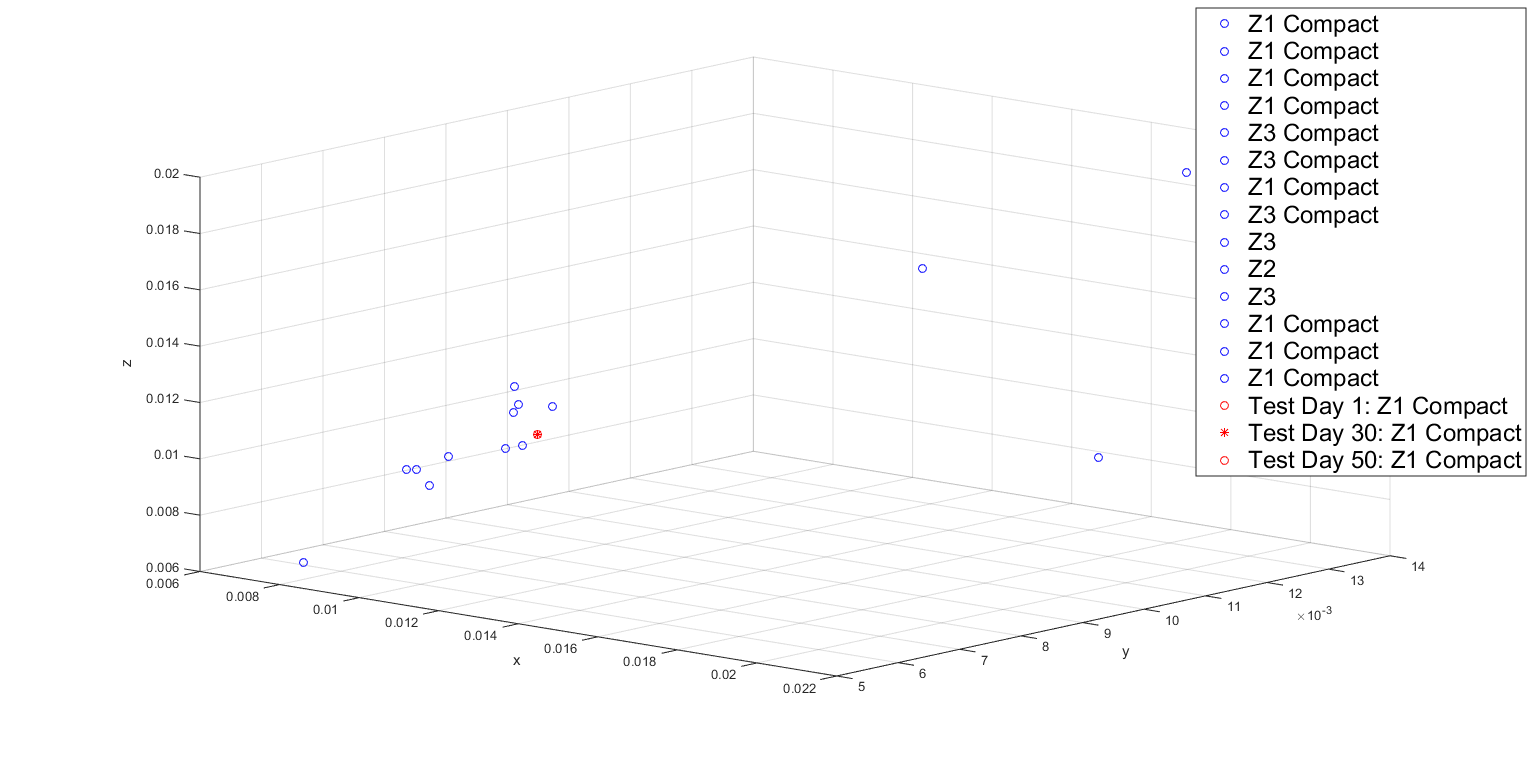
\includegraphics[scale=.3]{img/features/std_dev}
	\caption{Scatter-plot of standard deviation values of 12  \textit{Sony Xperia Z}-devices including one device with readings over a period of 50 days}
	\label{fig:feature:sddev}
\end{figure}

\section{Scatter-plot of average deviation values}
\begin{figure}[H]
	\centering
	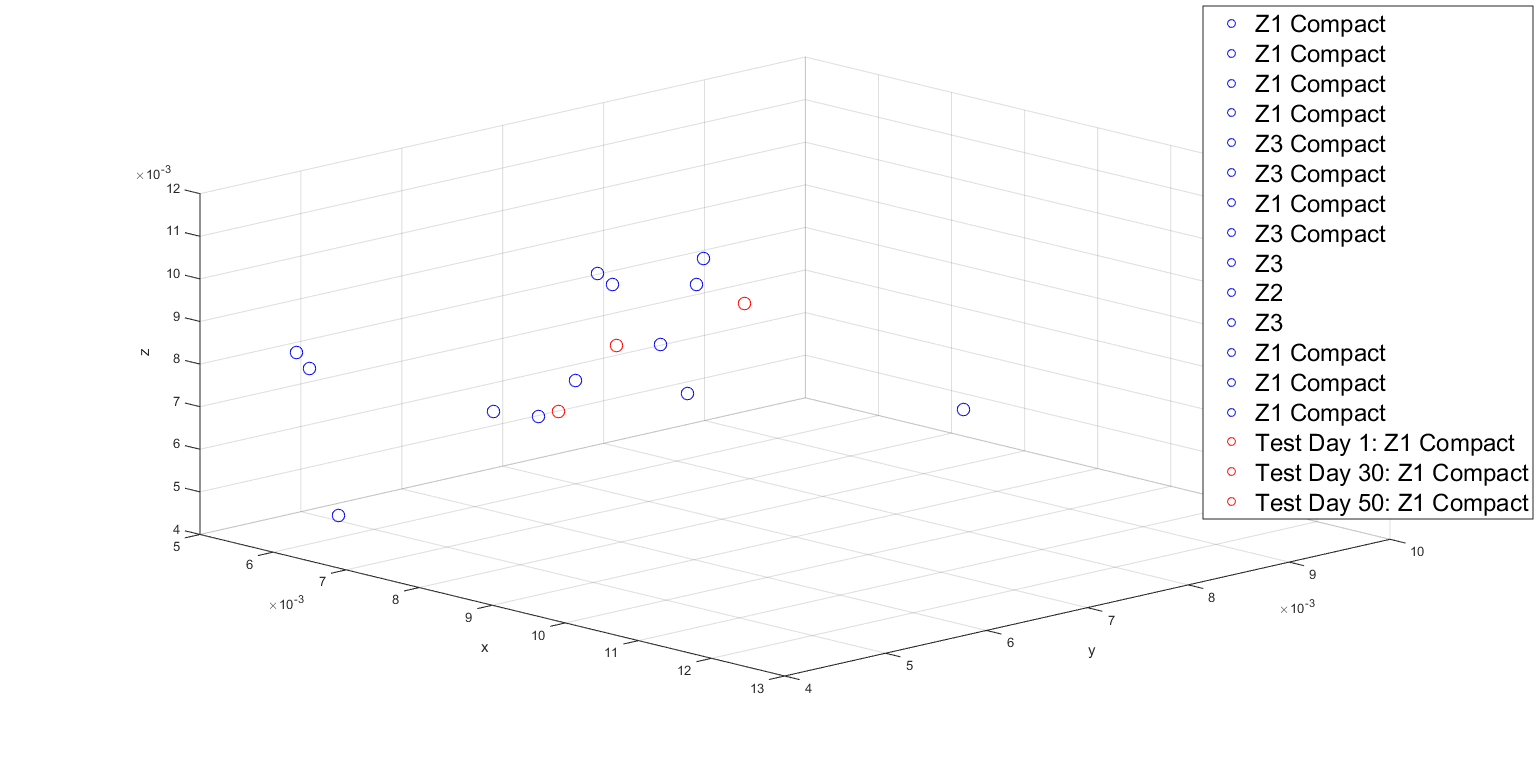
\includegraphics[scale=.3]{img/features/avg_dev}
	\caption{Scatter-plot of average deviation values of 12  \textit{Sony Xperia Z}-devices including one device with readings over a period of 50 days}
	\label{fig:feature:avgdev}
\end{figure}

\section{Scatter-plot of skewness values}
\begin{figure}[H]
	\centering
	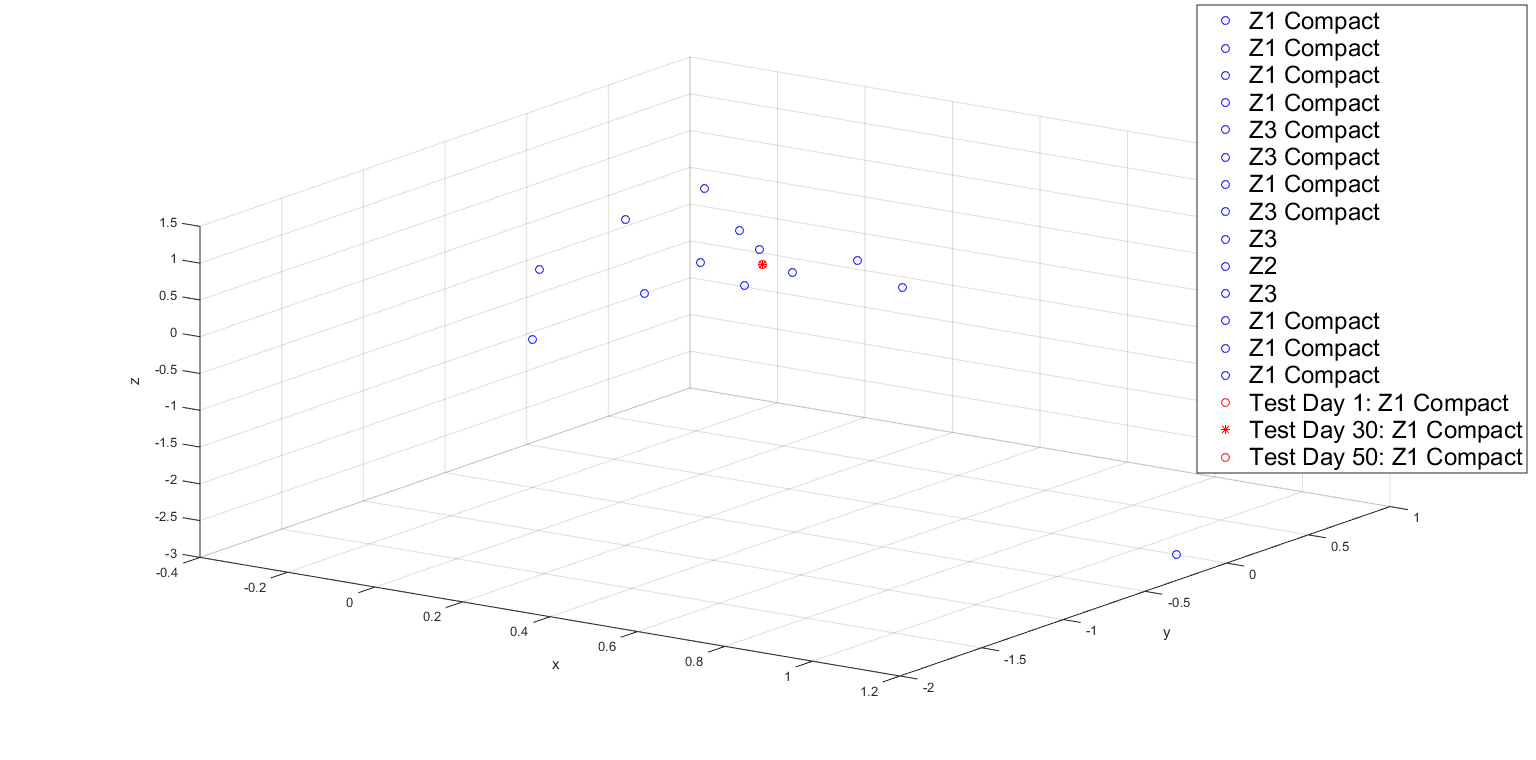
\includegraphics[scale=.3]{img/features/skew}
	\caption{Scatter-plot of skewness value of 12  \textit{Sony Xperia Z}-devices including one device with readings over a period of 50 days}
	\label{fig:feature:skew}
\end{figure}

\section{Scatter-plot of kurtosis values}
\begin{figure}[H]
	\centering
	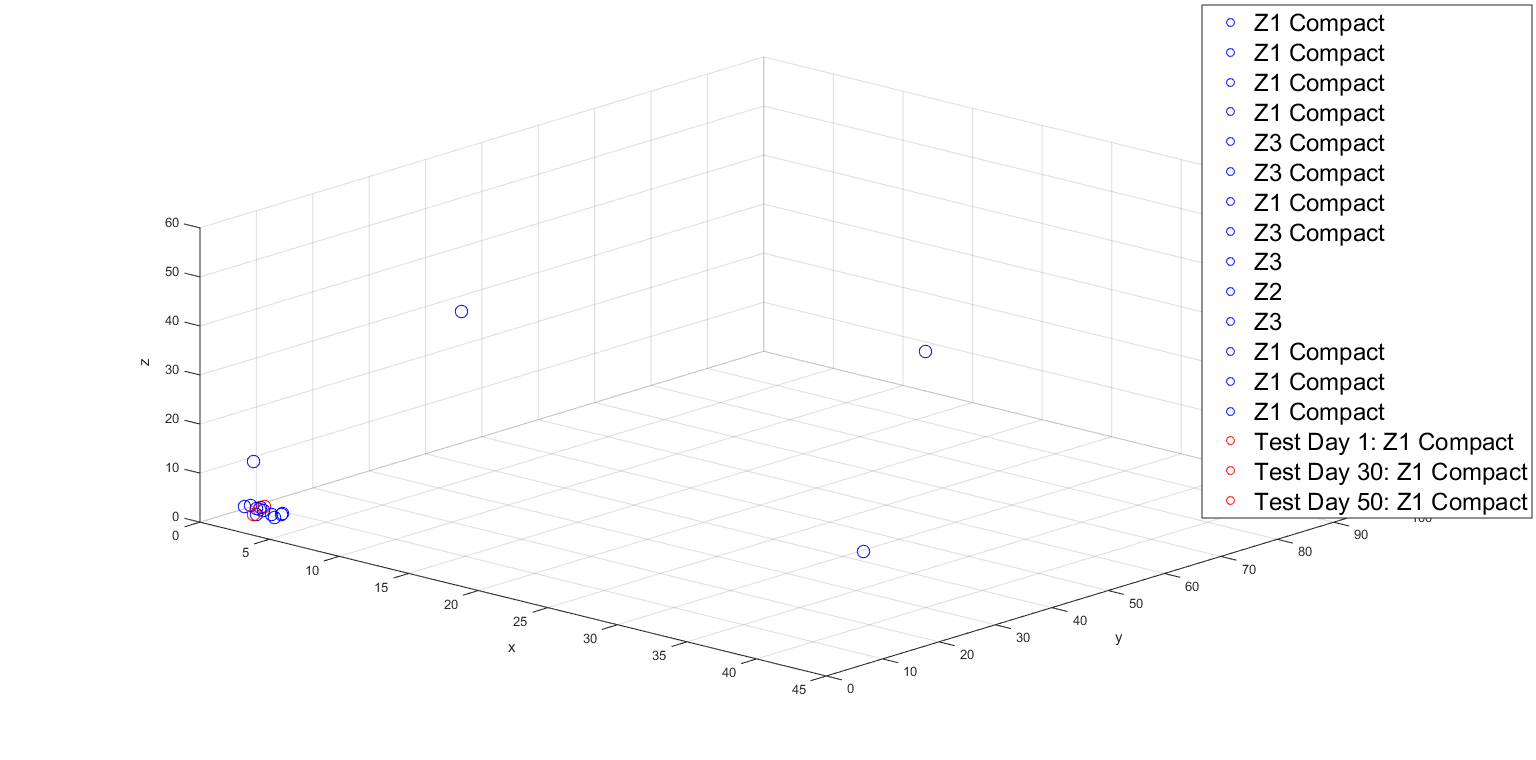
\includegraphics[scale=.3]{img/features/kurt}
	\caption{Scatter-plot of kurtosis values of 12  \textit{Sony Xperia Z}-devices including one device with readings over a period of 50 days}
	\label{fig:feature:kurt}
\end{figure}

\section{Scatter-plot of RMS values}
\begin{figure}[H]
	\centering
	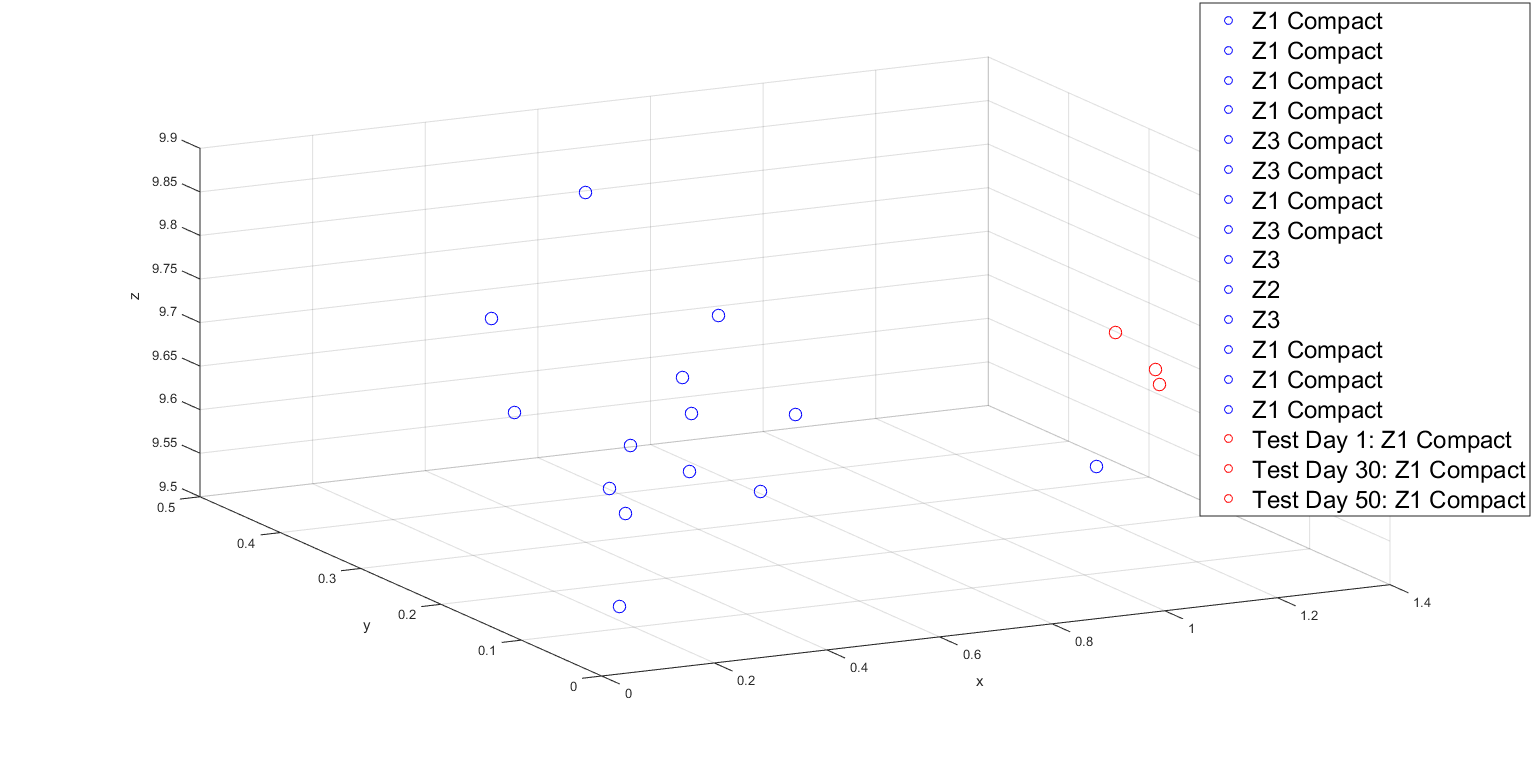
\includegraphics[scale=.3]{img/features/rms}
	\caption{Scatter-plot of RMS values of 12  \textit{Sony Xperia Z}-devices including one device with readings over a period of 50 days}
	\label{fig:feature:rms}
\end{figure}

\section{Scatter-plot of min values}
\begin{figure}[H]
	\centering
	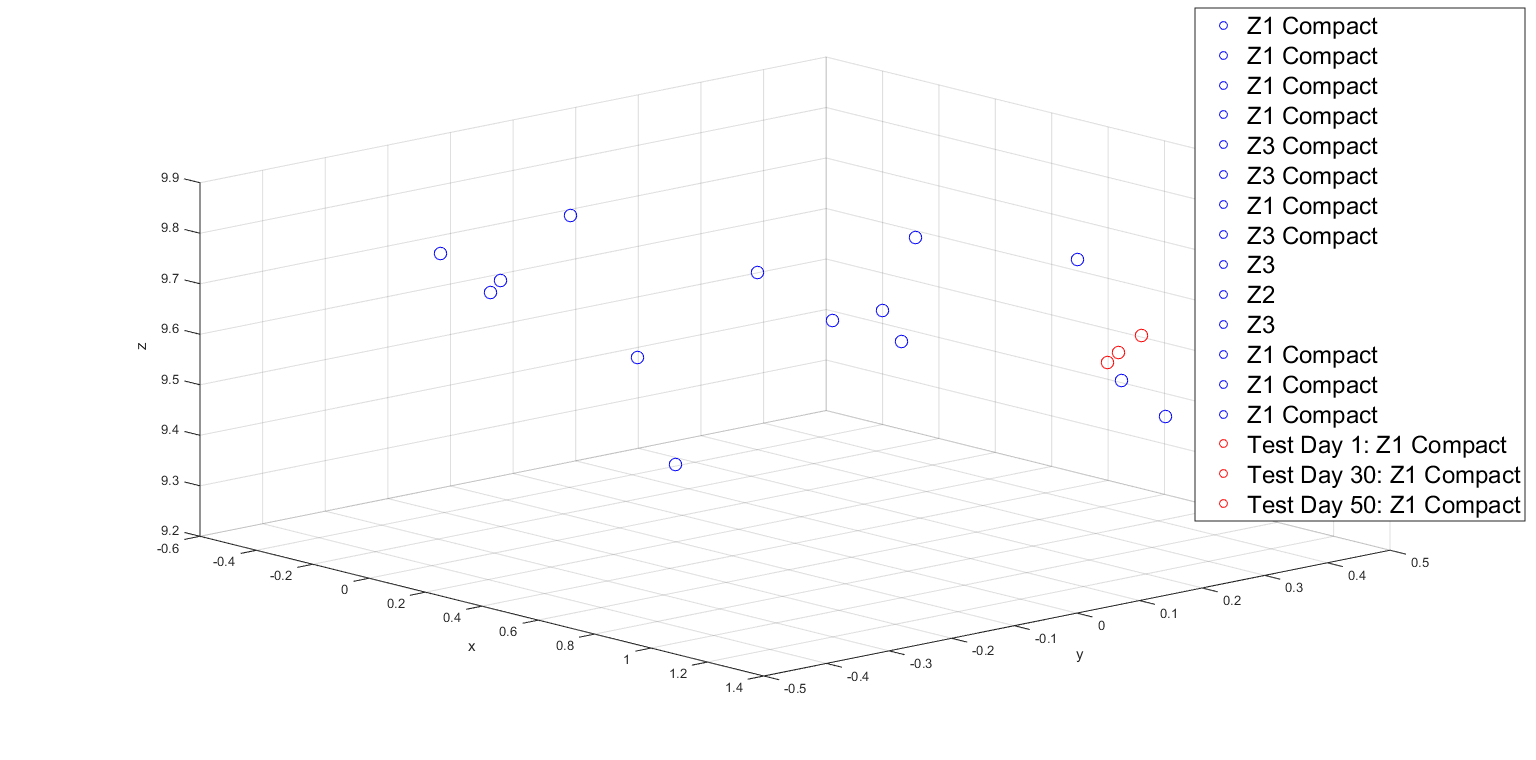
\includegraphics[scale=.3]{img/features/min}
	\caption{Scatter-plot of min values of 12  \textit{Sony Xperia Z}-devices including one device with readings over a period of 50 days}
	\label{fig:feature:min}
\end{figure}

\section{Scatter-plot of max values}
\begin{figure}[H]
	\centering
	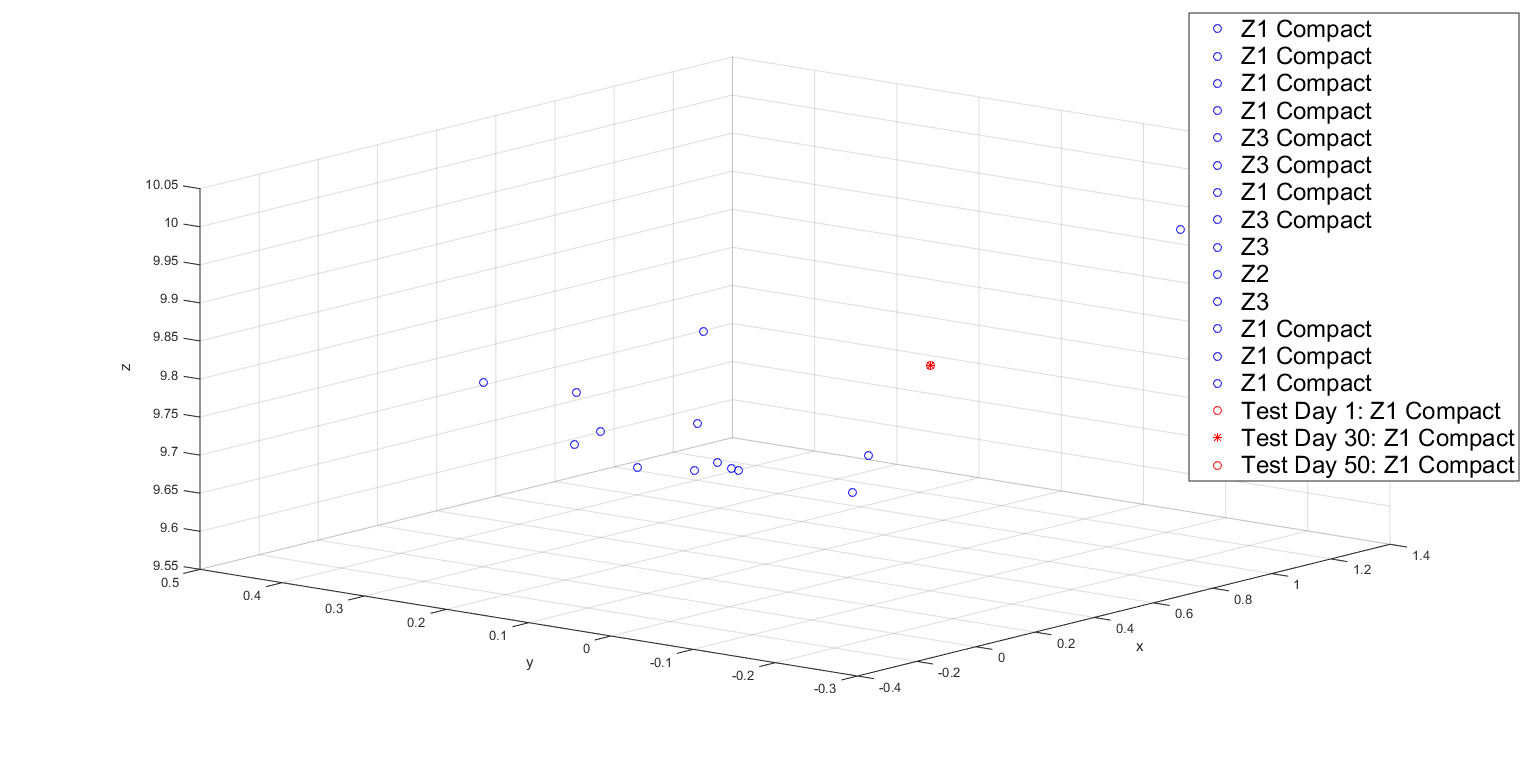
\includegraphics[scale=.3]{img/features/max}
	\caption{Scatter-plot of max value of 12  \textit{Sony Xperia Z}-devices including one device with readings over a period of 50 days}
	\label{fig:feature:max}
\end{figure}


